\appendix

\section{Additional Coke-Can Rollout Visualizations}

Figure~\ref{fig:appendix_coke_rollouts} shows representative rollouts from the Coke-can force-steering experiments. For each condition, we visualize the RGB observation, the masked gripper input used by ForceLens, and the corresponding edge-only input at multiple points in the rollout. Each panel overlays the ForceLens predicted force for the corresponding time step.

\begin{figure*}[p]
    \centering
    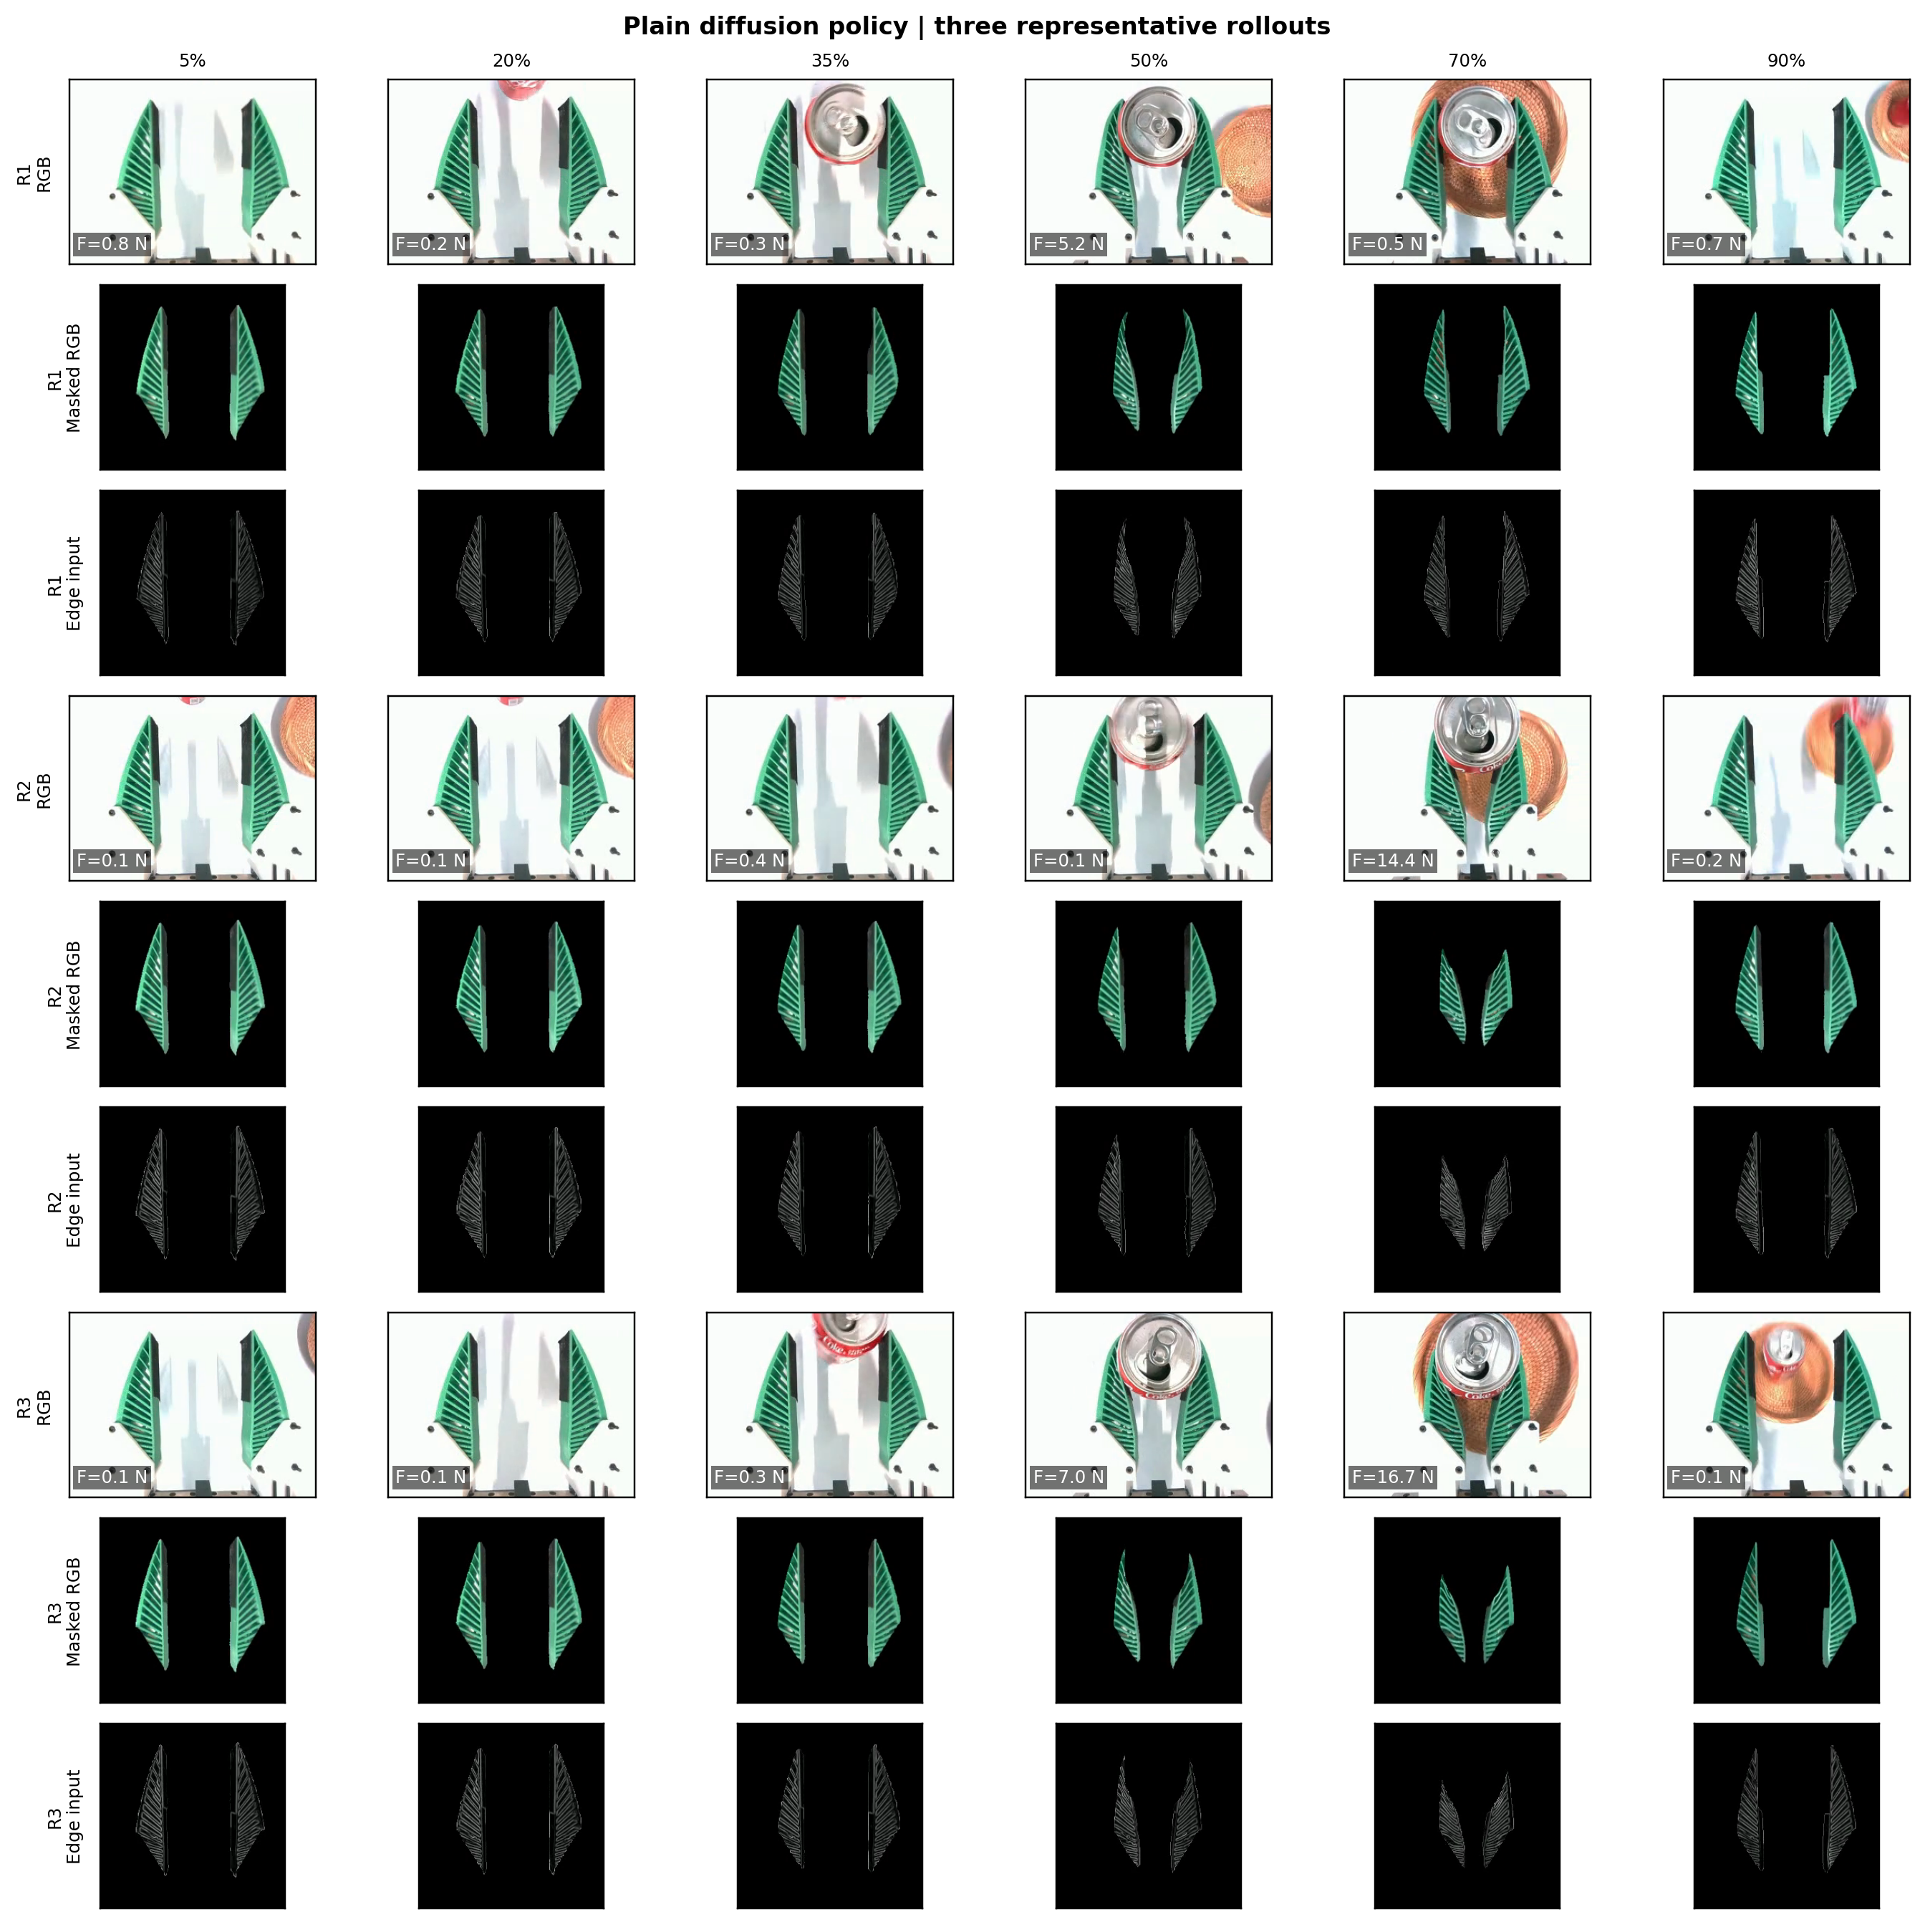
\includegraphics[width=\linewidth]{reports/coke_force_steering/appendix/appendix_grab_coke_empty_dp_three_rollouts.png}
    \\[-0.25em]{\small Plain diffusion policy; peak estimated forces 8.13, 15.22, 18.57\,N.}
    \vspace{0.5em}
    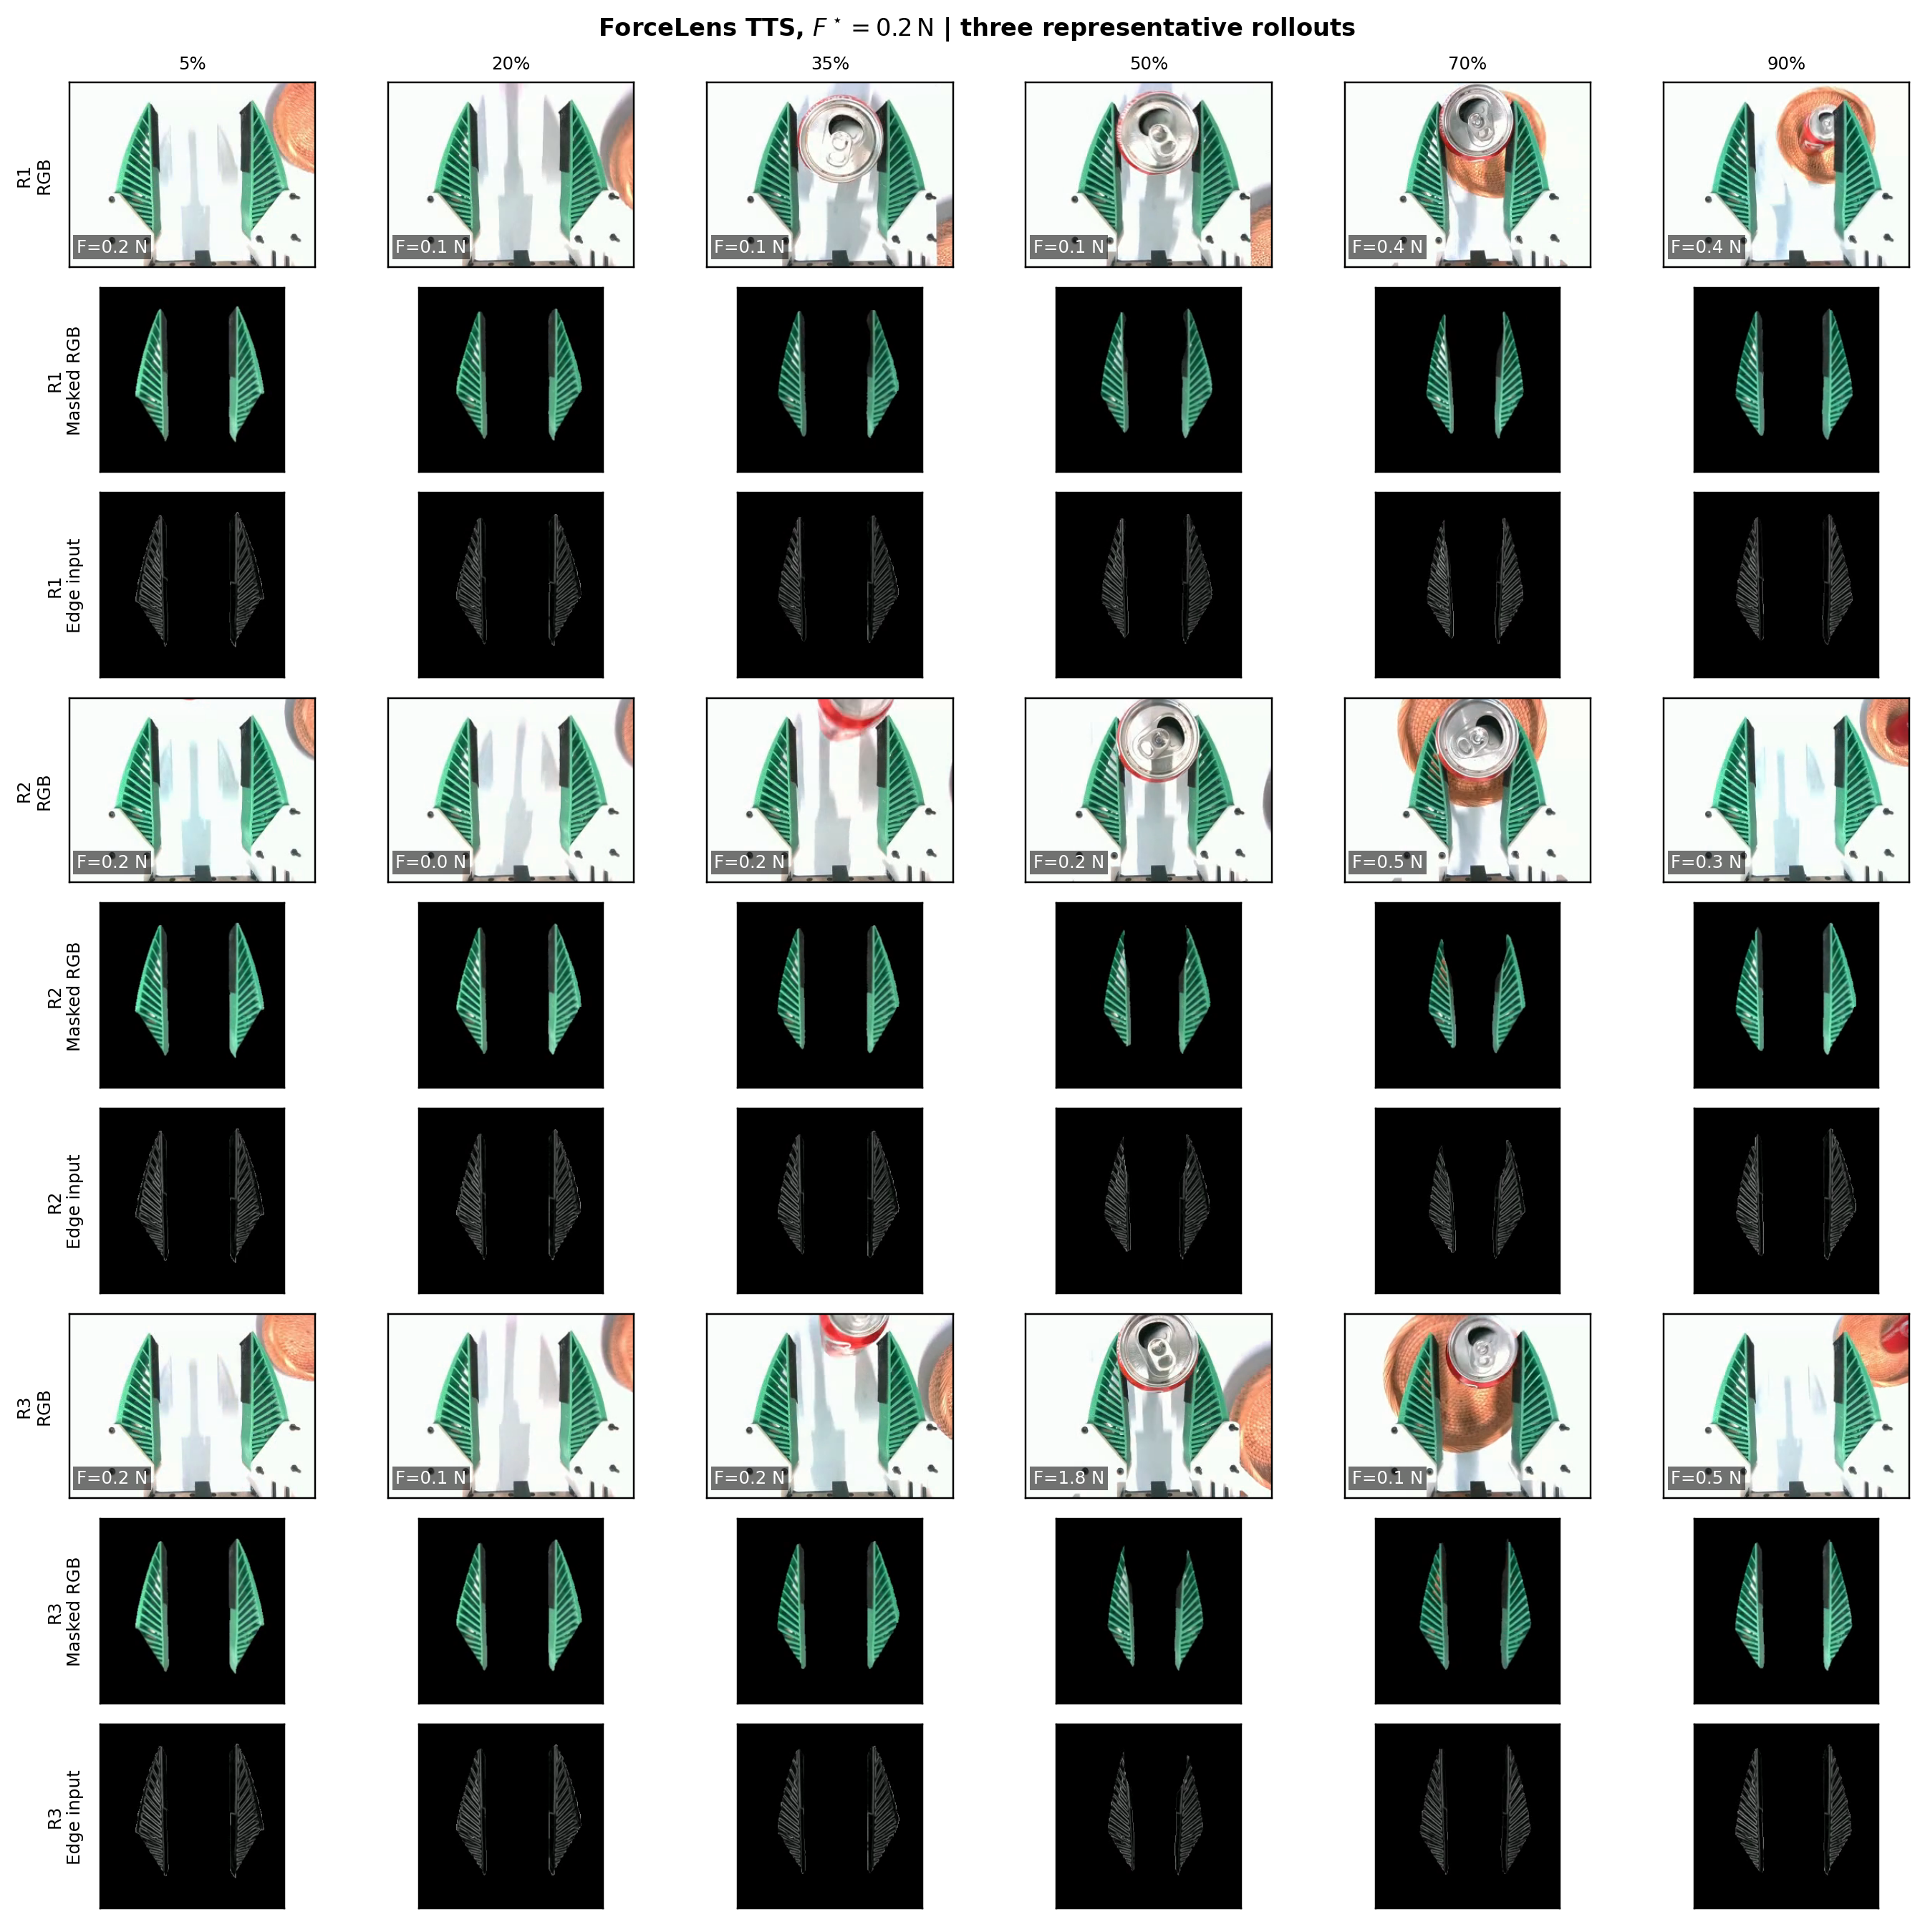
\includegraphics[width=\linewidth]{reports/coke_force_steering/appendix/appendix_grab_coke_empty_0_2N_three_rollouts.png}
    \\[-0.25em]{\small ForceLens TTS, $F^\star=0.2\,\mathrm{N}$; peak estimated forces 2.12, 3.18, 4.25\,N.}
    \vspace{0.5em}
    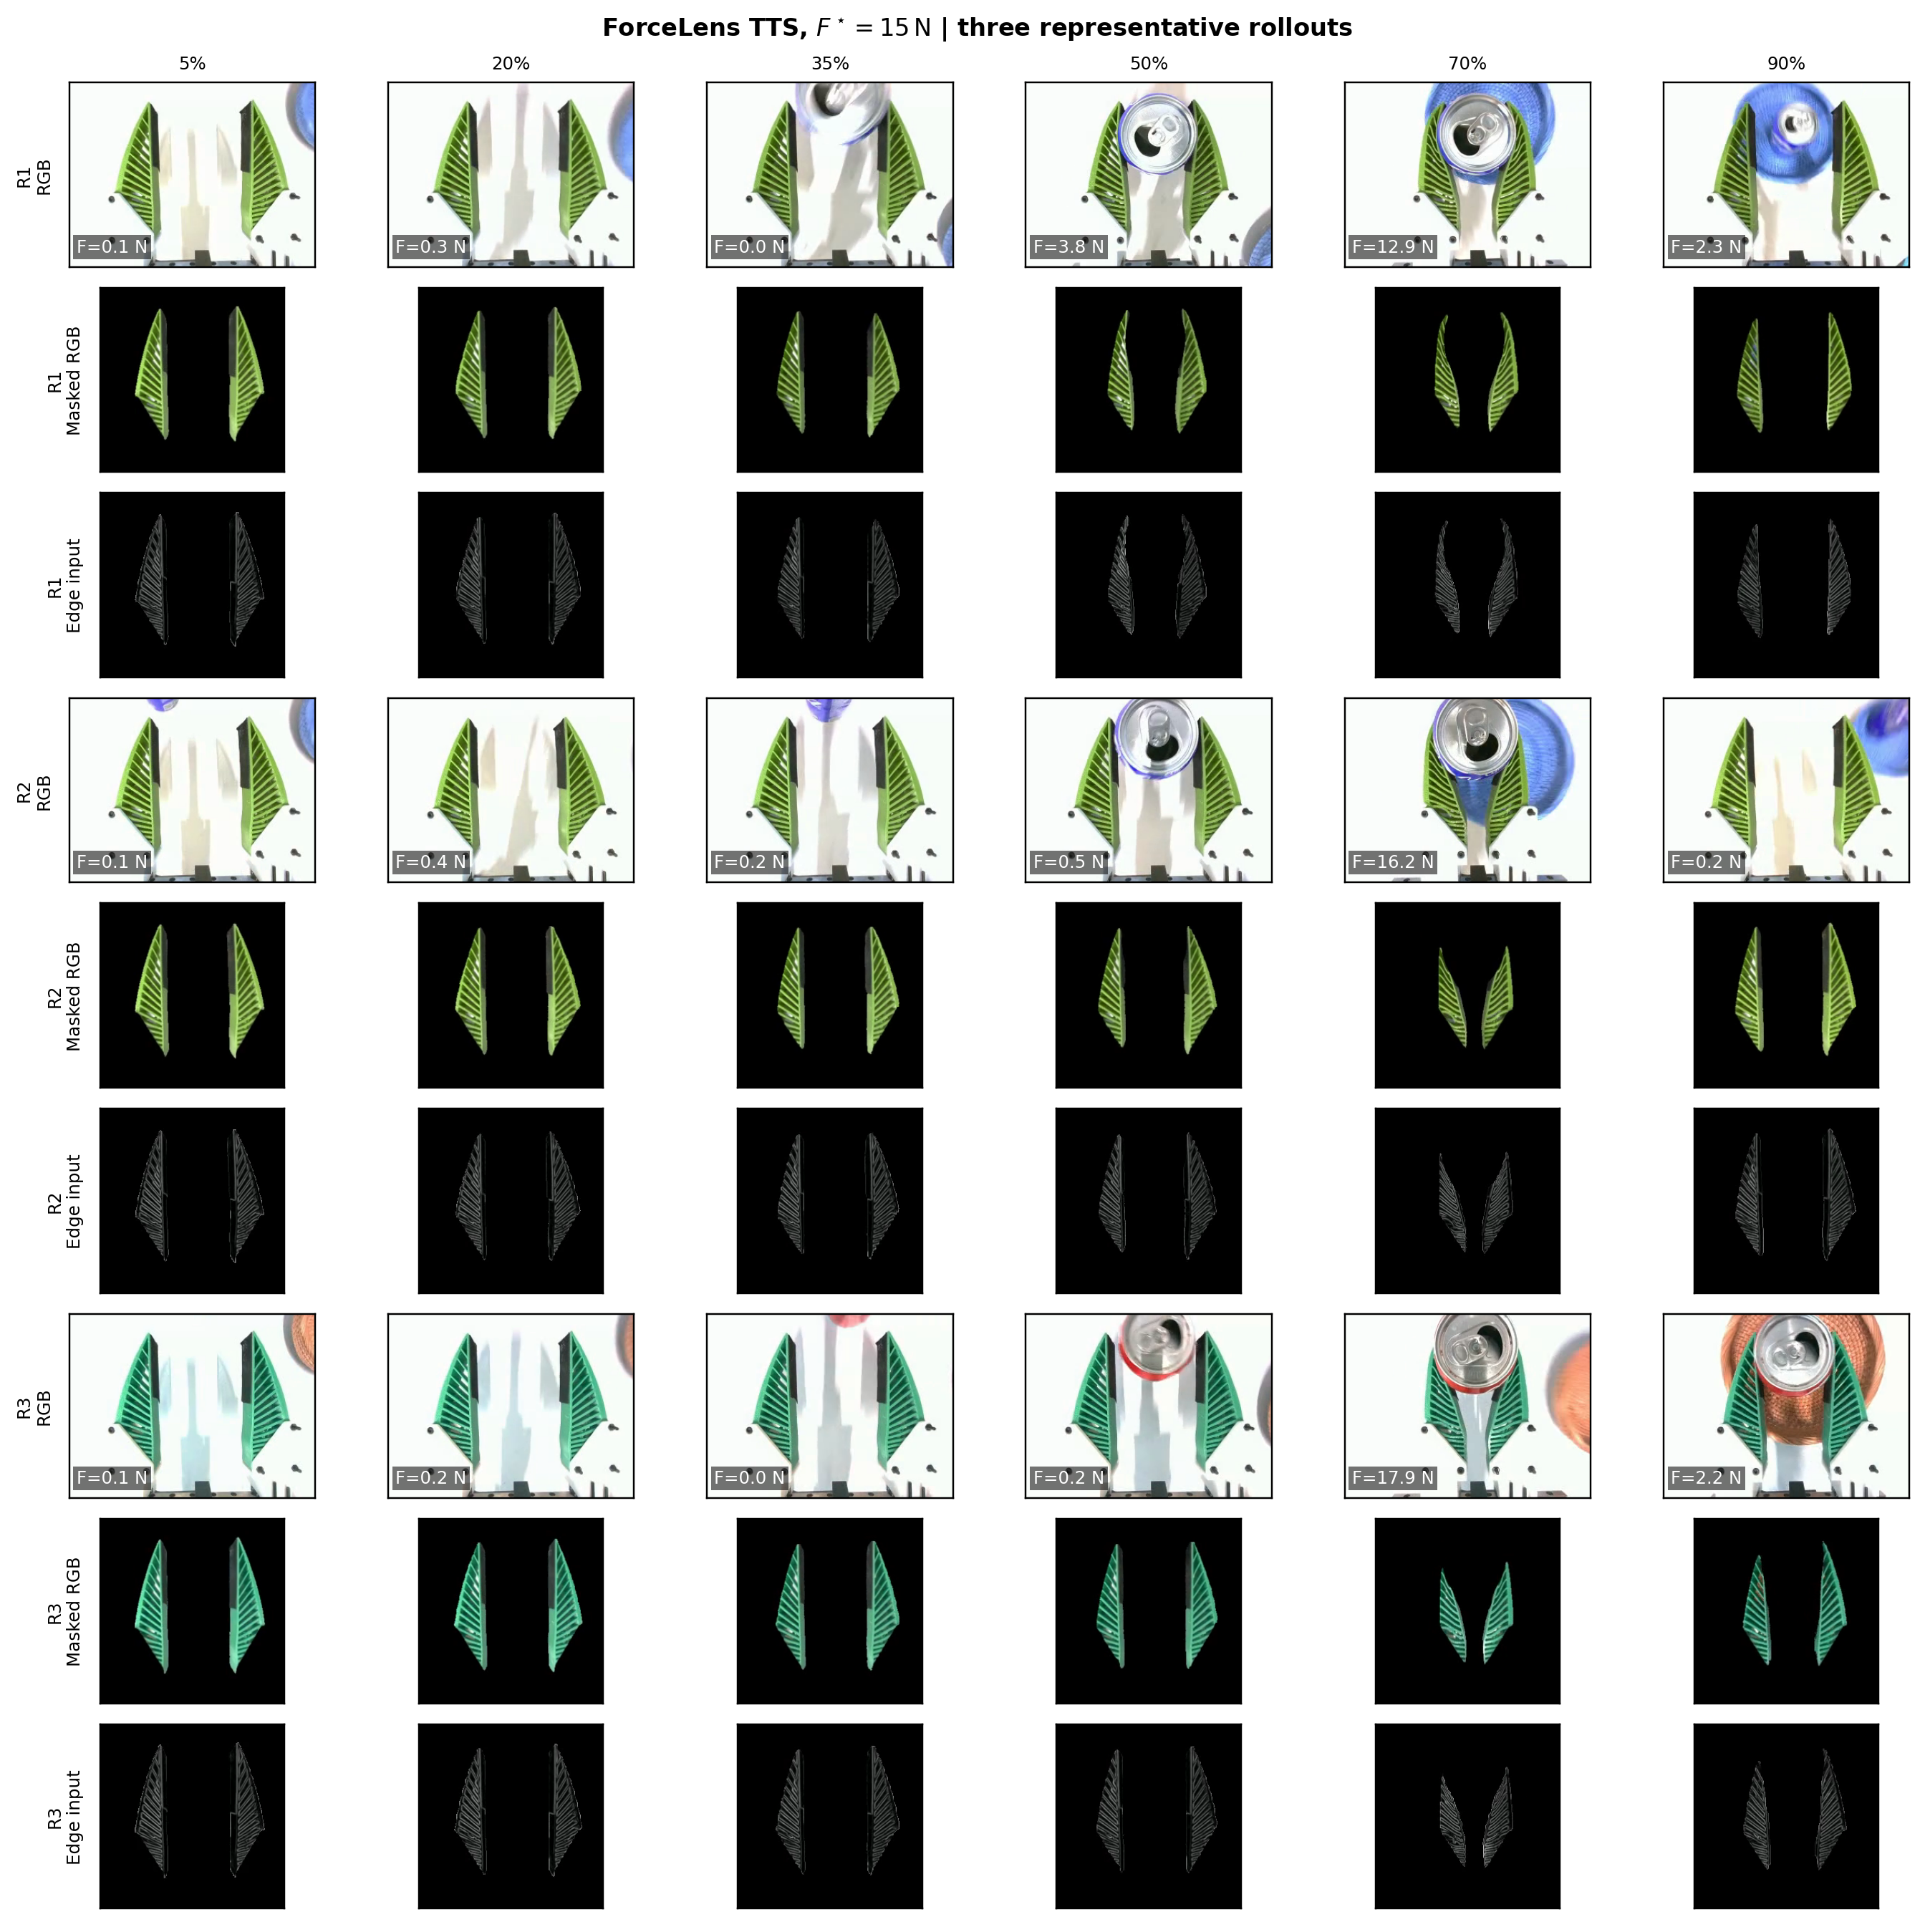
\includegraphics[width=\linewidth]{reports/coke_force_steering/appendix/appendix_grab_coke_empty_15_0N_three_rollouts.png}
    \\[-0.25em]{\small ForceLens TTS, $F^\star=15\,\mathrm{N}$; peak estimated forces 15.84, 16.38, 18.21\,N.}
    \vspace{0.5em}
    \caption{Representative Coke-can rollouts used in the force-steering evaluation. Each block shows one condition, with three representative rollouts. Columns denote rollout progress and rows denote RGB, masked RGB, and edge-only ForceLens inputs. White labels indicate predicted force.}
    \label{fig:appendix_coke_rollouts}
\end{figure*}
